\section{Travaux de modélisations} 
\subsection{Modification du Modèle Conceptuelle de Donnée}

Pour permettre l'enregistrement des emprunts ainsi que des lieux d'emprunts il a fallu ajouter une table \emph{Location\_E} (qui indique le lieu de location) ainsi qu'un table \emph{Bilioteque} (qui indique le lieu d'emprunt) au MCD déjà existant dans Royal\_.
De même nous avons rajouté un boolean \emph{Enprunté\_A} à la table \emph{Album} afin d'indiquer si un livre est emprunté ou nous appartient.

\begin{figure}[h!]
\begin{center}
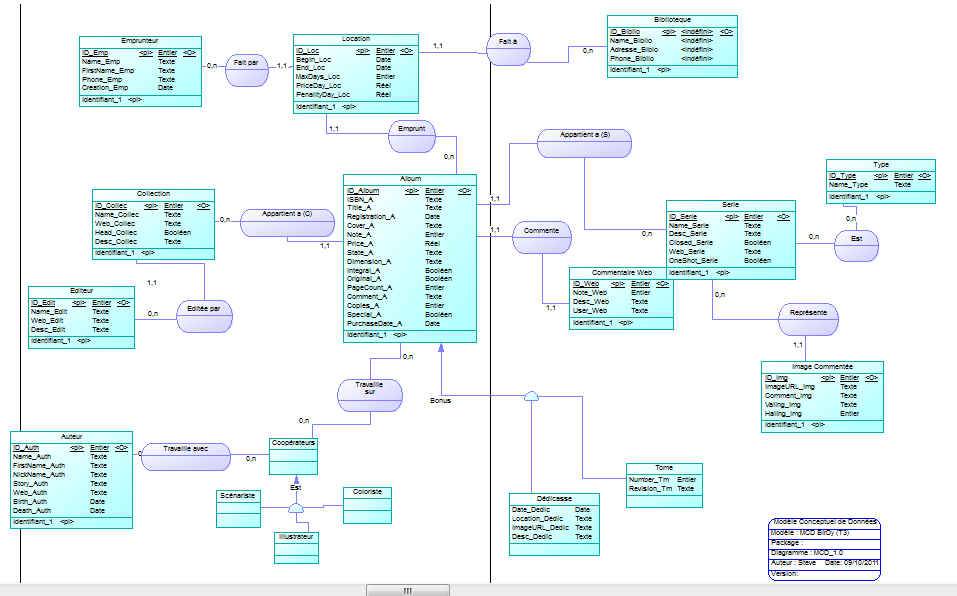
\includegraphics[width=13cm]{MCD_Royal_Modif.png}
\end{center}
\end{figure}
\newpage{} 

\subsection{Modèle conceptuel de traitement}

Le MCT ci-dessous montre les différents traitement effectués dans Royal\_. 
Ces traitements seront présentés en fonction de leurs prioritées.
Nous pouvons observer tout d'abord la synchronisation d'\emph{ISBN} (sur le client pc) présent dans la boite mail ainsi que la capture d'\emph{ISBNs} (sur le client android).
Ensuite nous pouvons voir que la synchronisation si les albums sont loués une demande d'informations sur l'emprunt est exécuté (cette demande d'ajout d'informations sur l'emprunt peut aussi etre effectué indépendamment).
A coté nous pouvons voir le MCT concernant la vérification des albums à rendre.
Enfin les deux derniers MCT traitent de la synchronisation des Albums déjà présents sur le client pc avec le client android.

%\begin{wrapfigure}[1]{l}{14cm}
%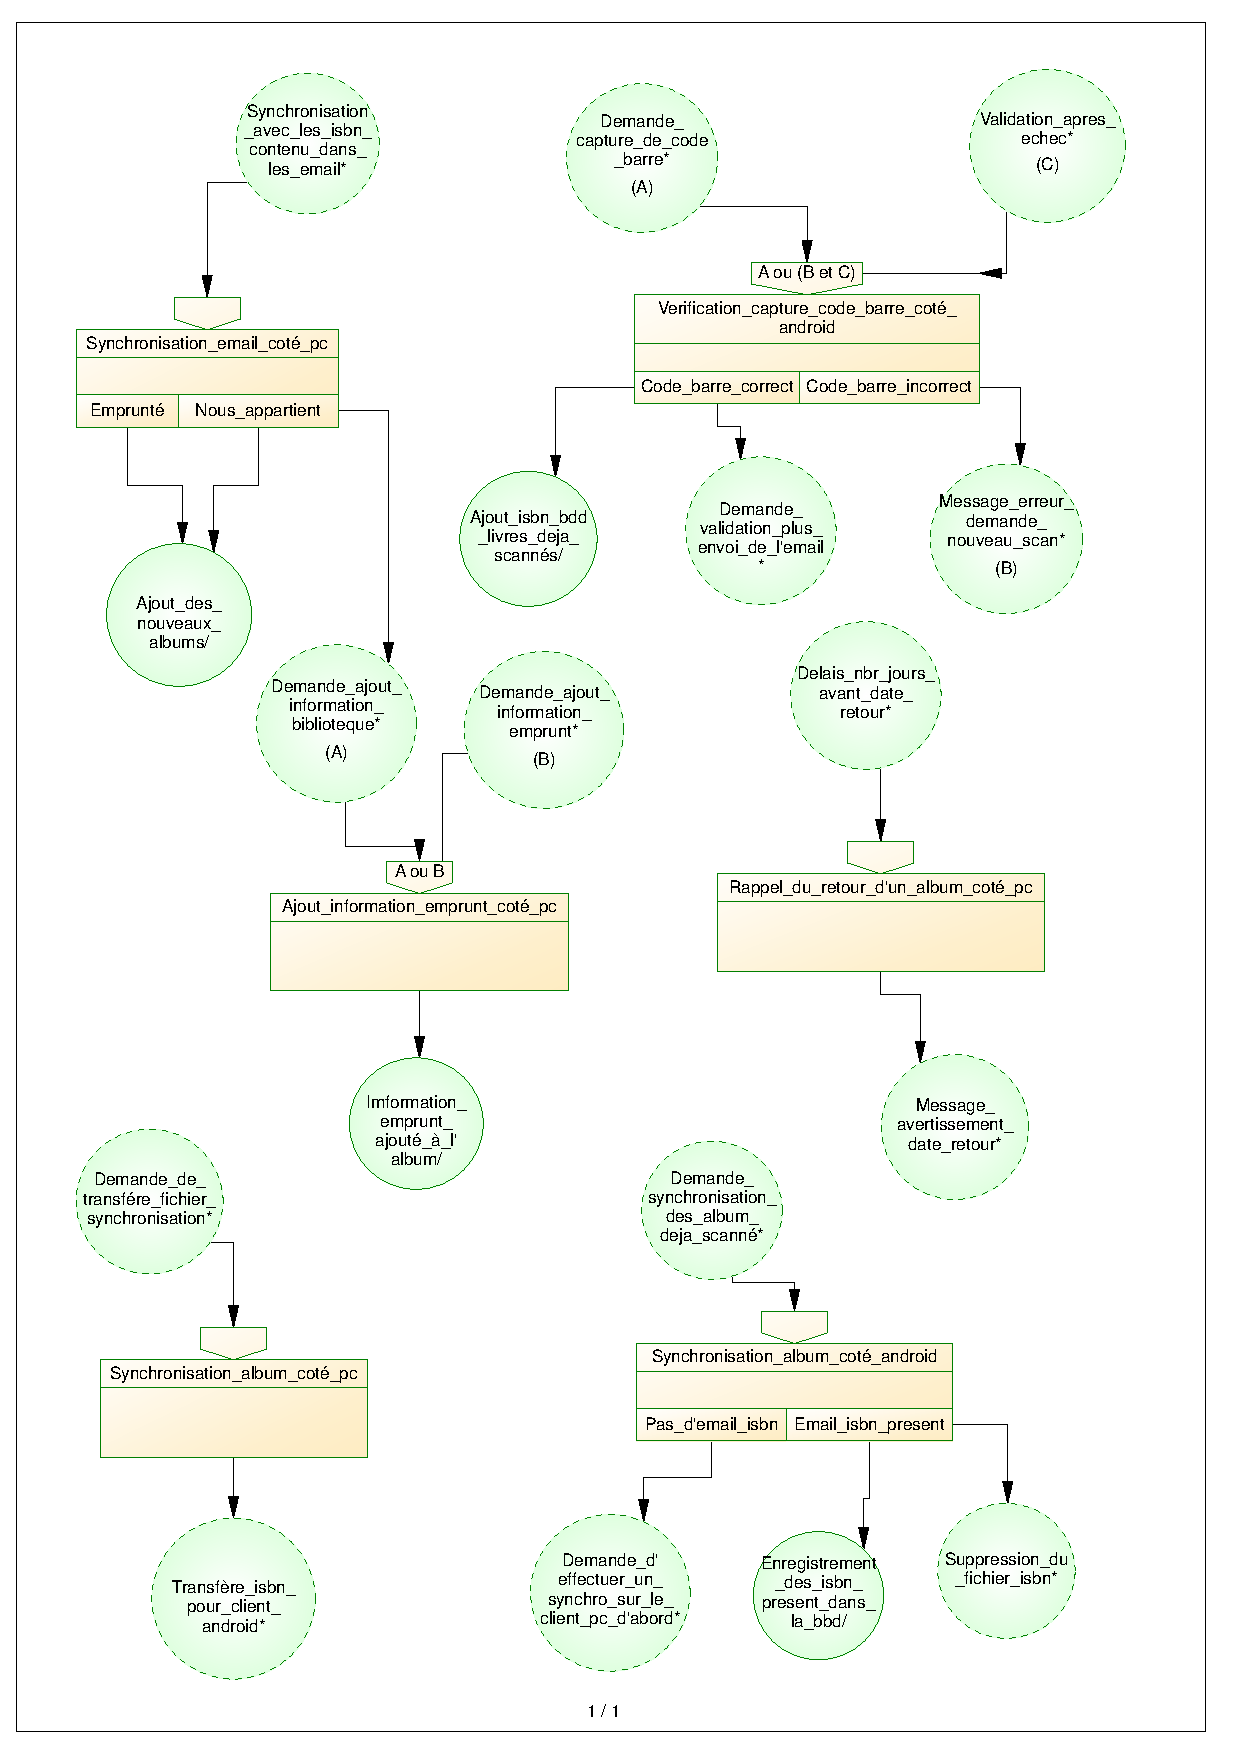
\includegraphics[width=14cm]{MCT_Royal.pdf}
%\end{wrapfigure}
%\clearpage{}

\begin{figure}[h!]
\begin{center}
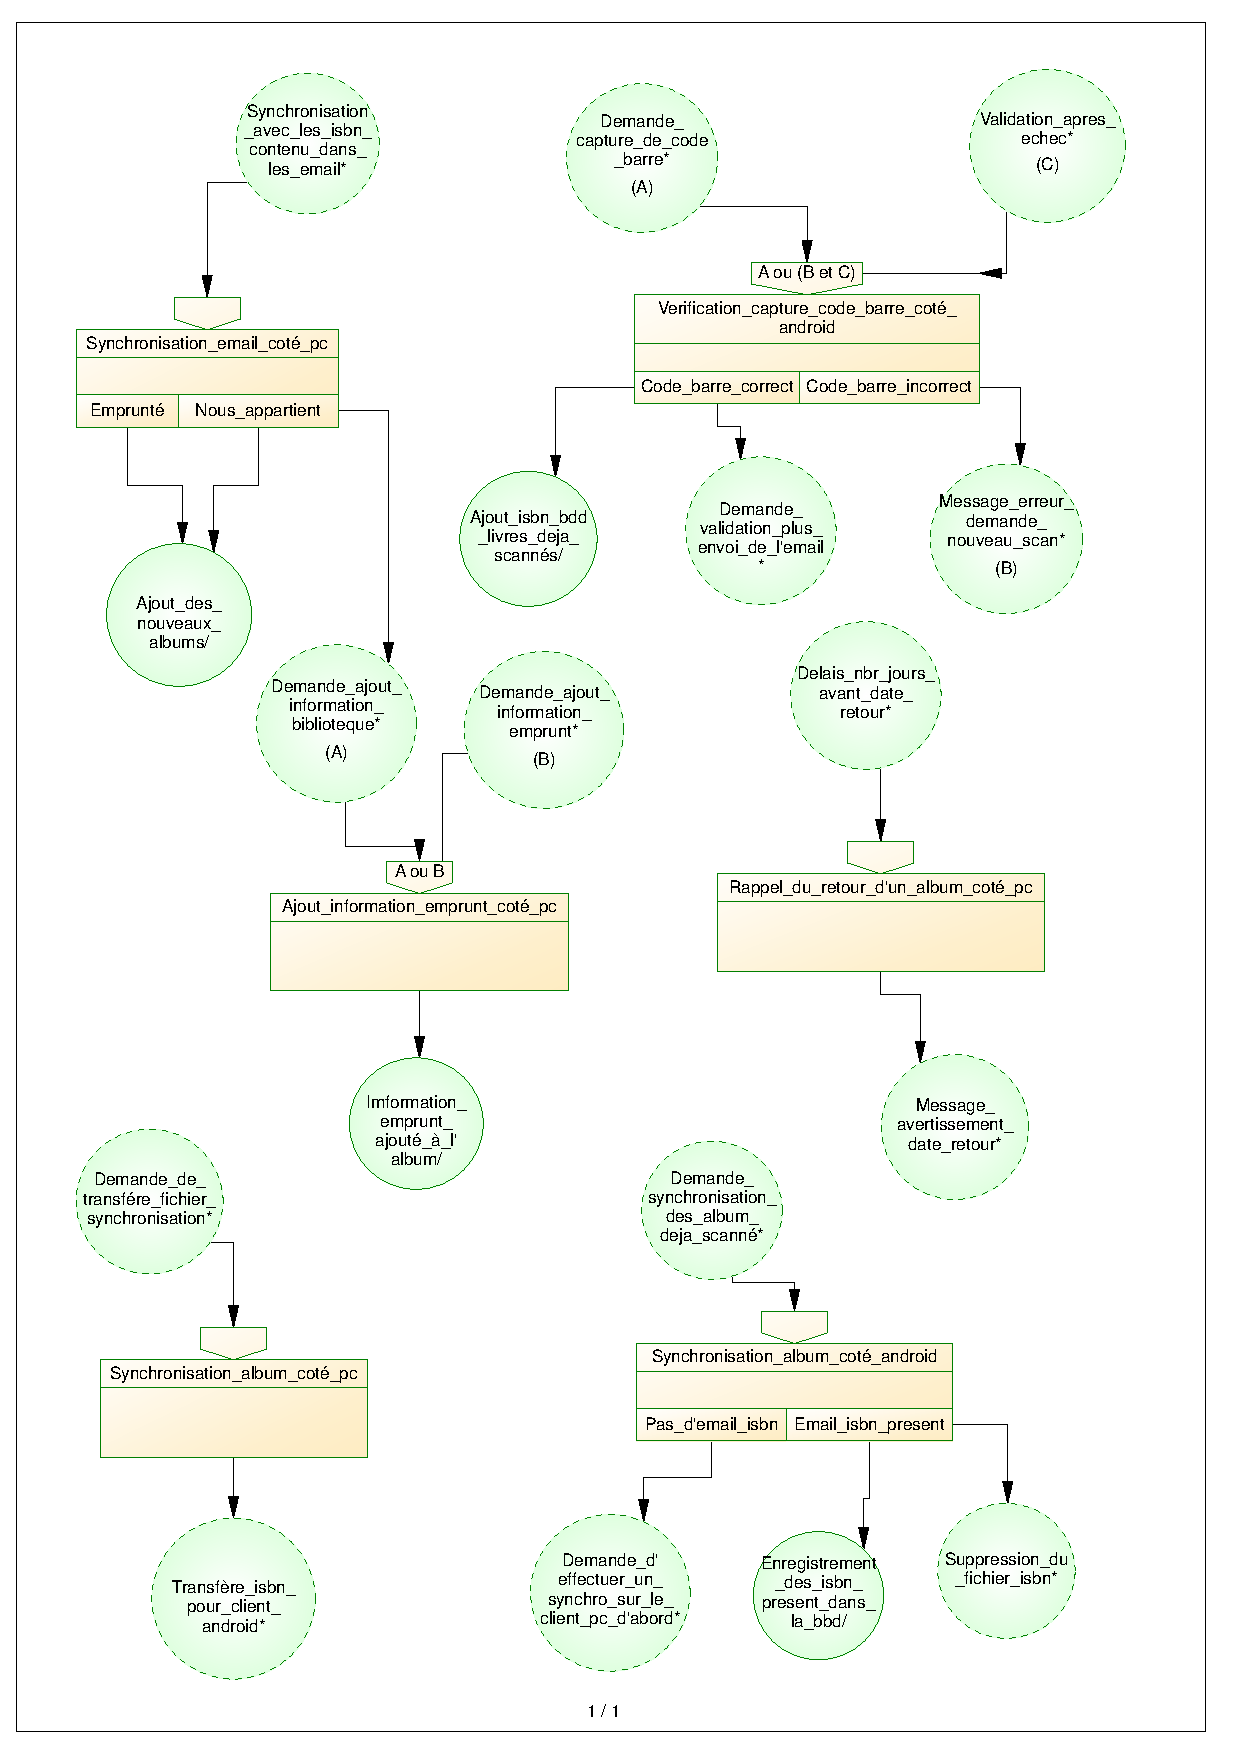
\includegraphics[width=14cm]{MCT_Royal.pdf}
\end{center}
\end{figure}
\newpage{}

\subsection{Diagrammes d'activités}
\subsubsection{Application PC}

\begin{figure}[h!]
\begin{center}
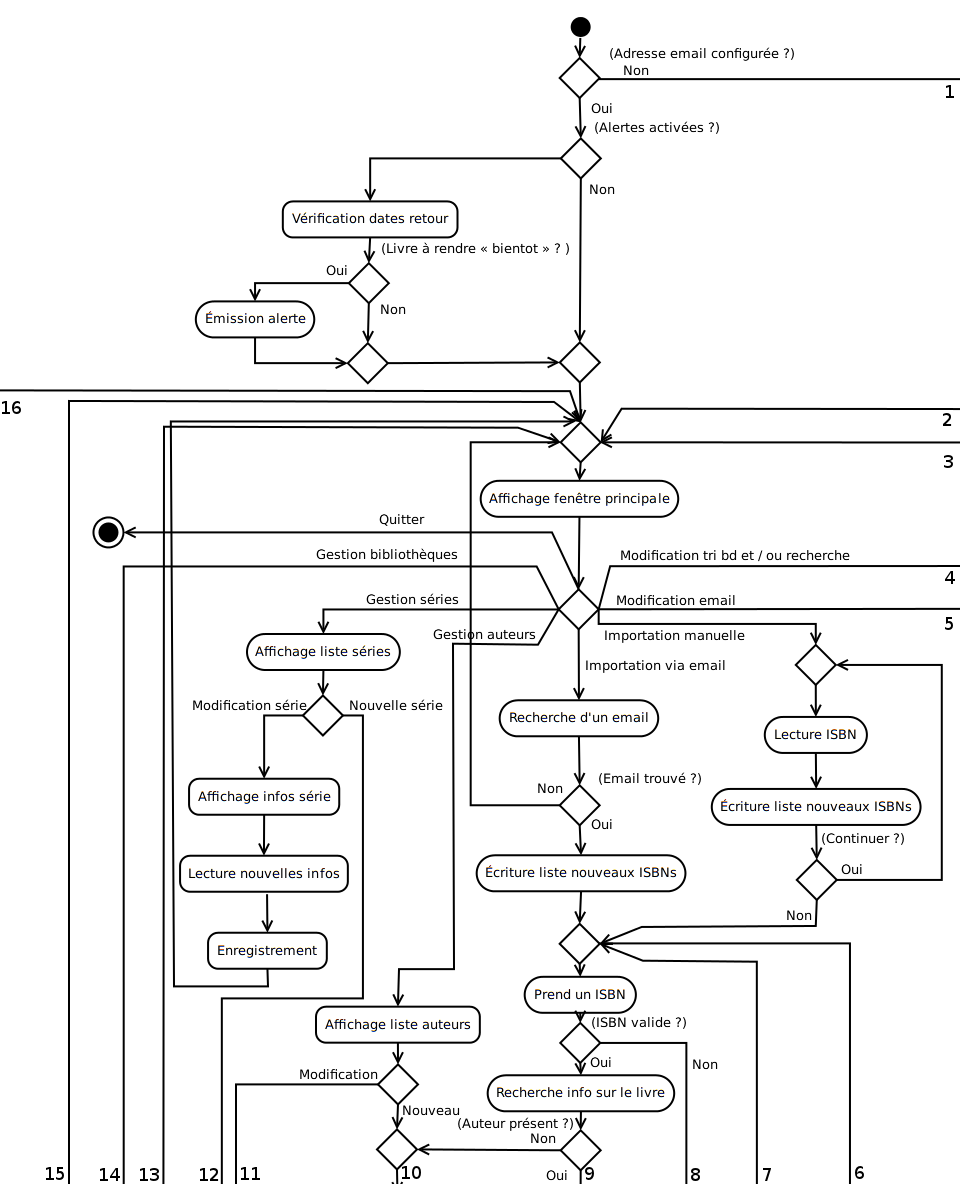
\includegraphics[width=16cm, height=19cm]{uml/appli_pc/p1.png}
\end{center}
\end{figure}
\newpage{}

\begin{figure}[h!]
\begin{center}
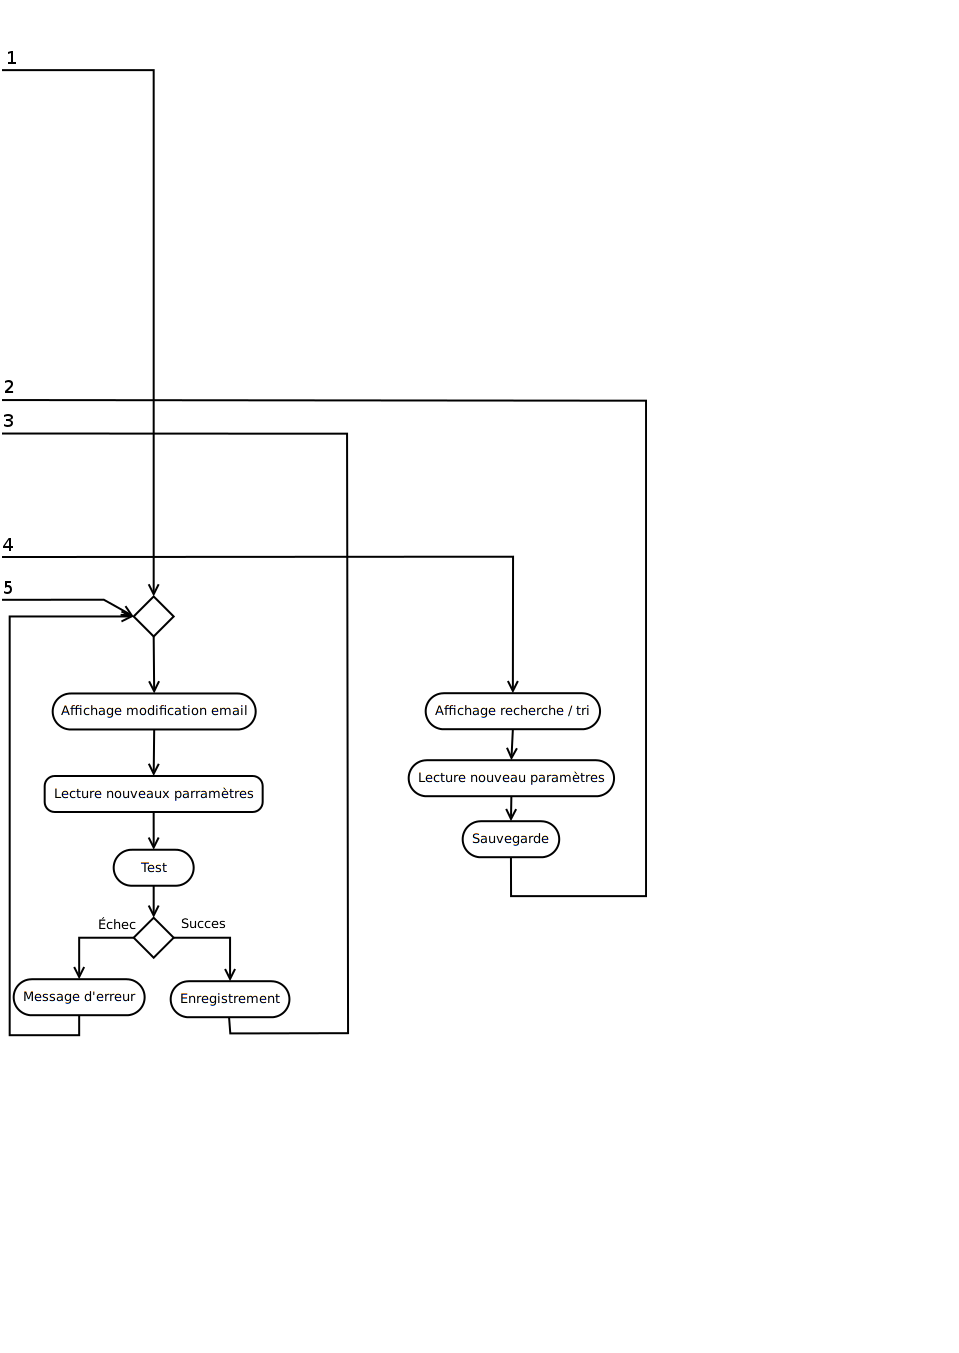
\includegraphics[width=16cm]{uml/appli_pc/p2.png}
\end{center}
\end{figure}
\newpage{}

\begin{figure}[h!]
\begin{center}
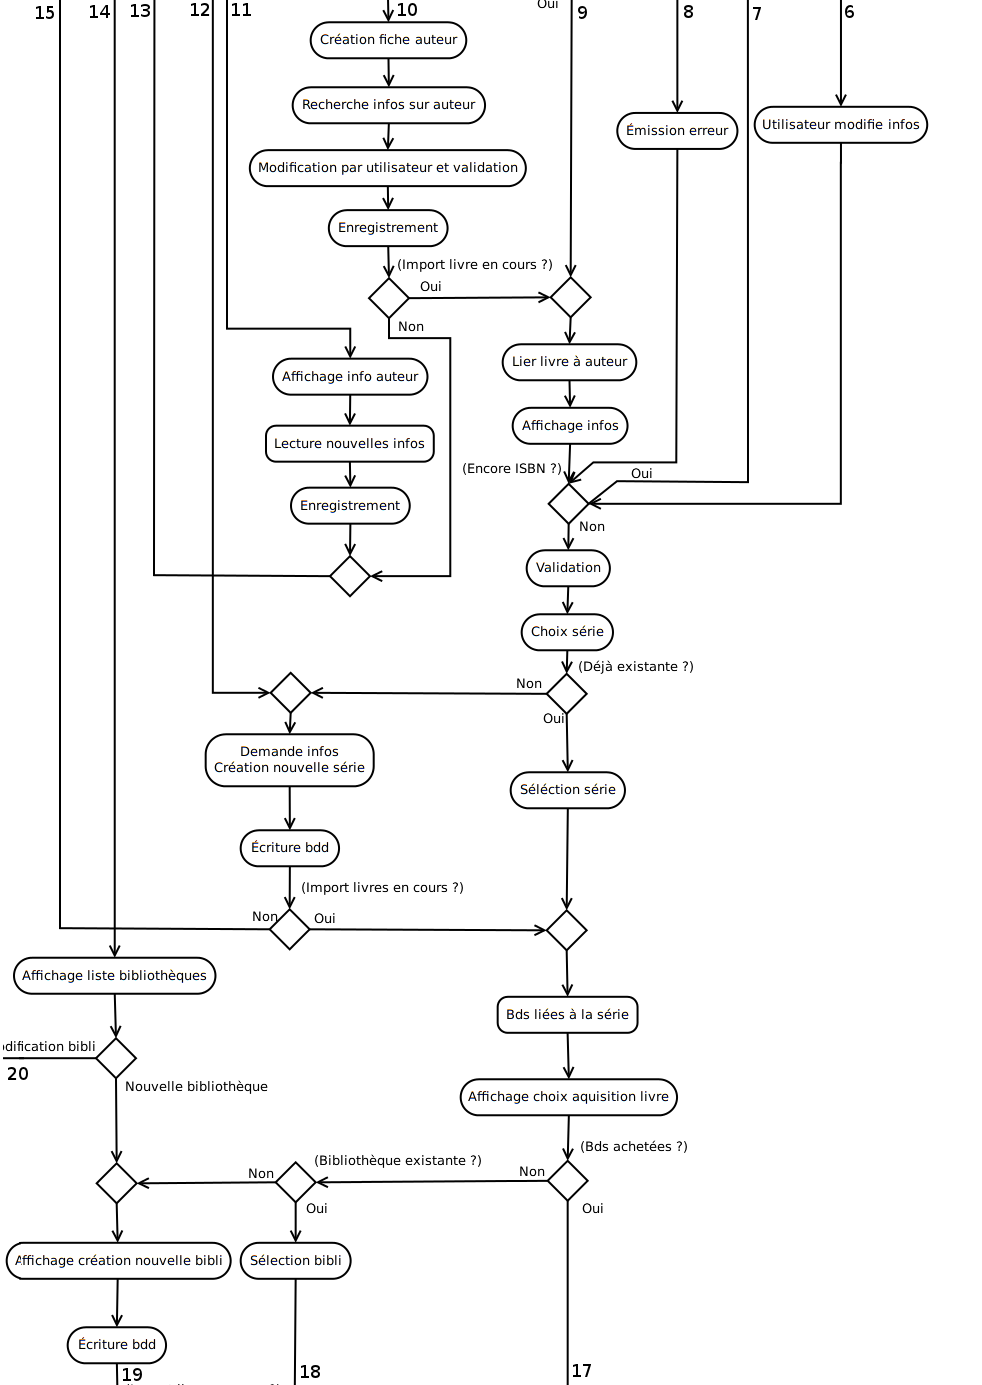
\includegraphics[width=16cm]{uml/appli_pc/p3.png}
\end{center}
\end{figure}
\newpage{}

\begin{figure}[t!]
\begin{center}
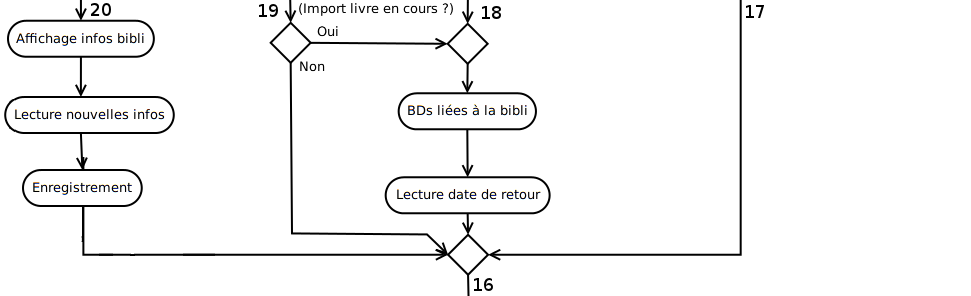
\includegraphics[width=16cm]{uml/appli_pc/p4.png}
\end{center}
\end{figure}

Une version plus lisible est disponible à l'adresse suivante : 
\emph{www.spyzone.fr/modules/images/application\_pc.png}
\newpage{}

\subsubsection{Application Android}
\begin{figure}[h!]
\begin{center}
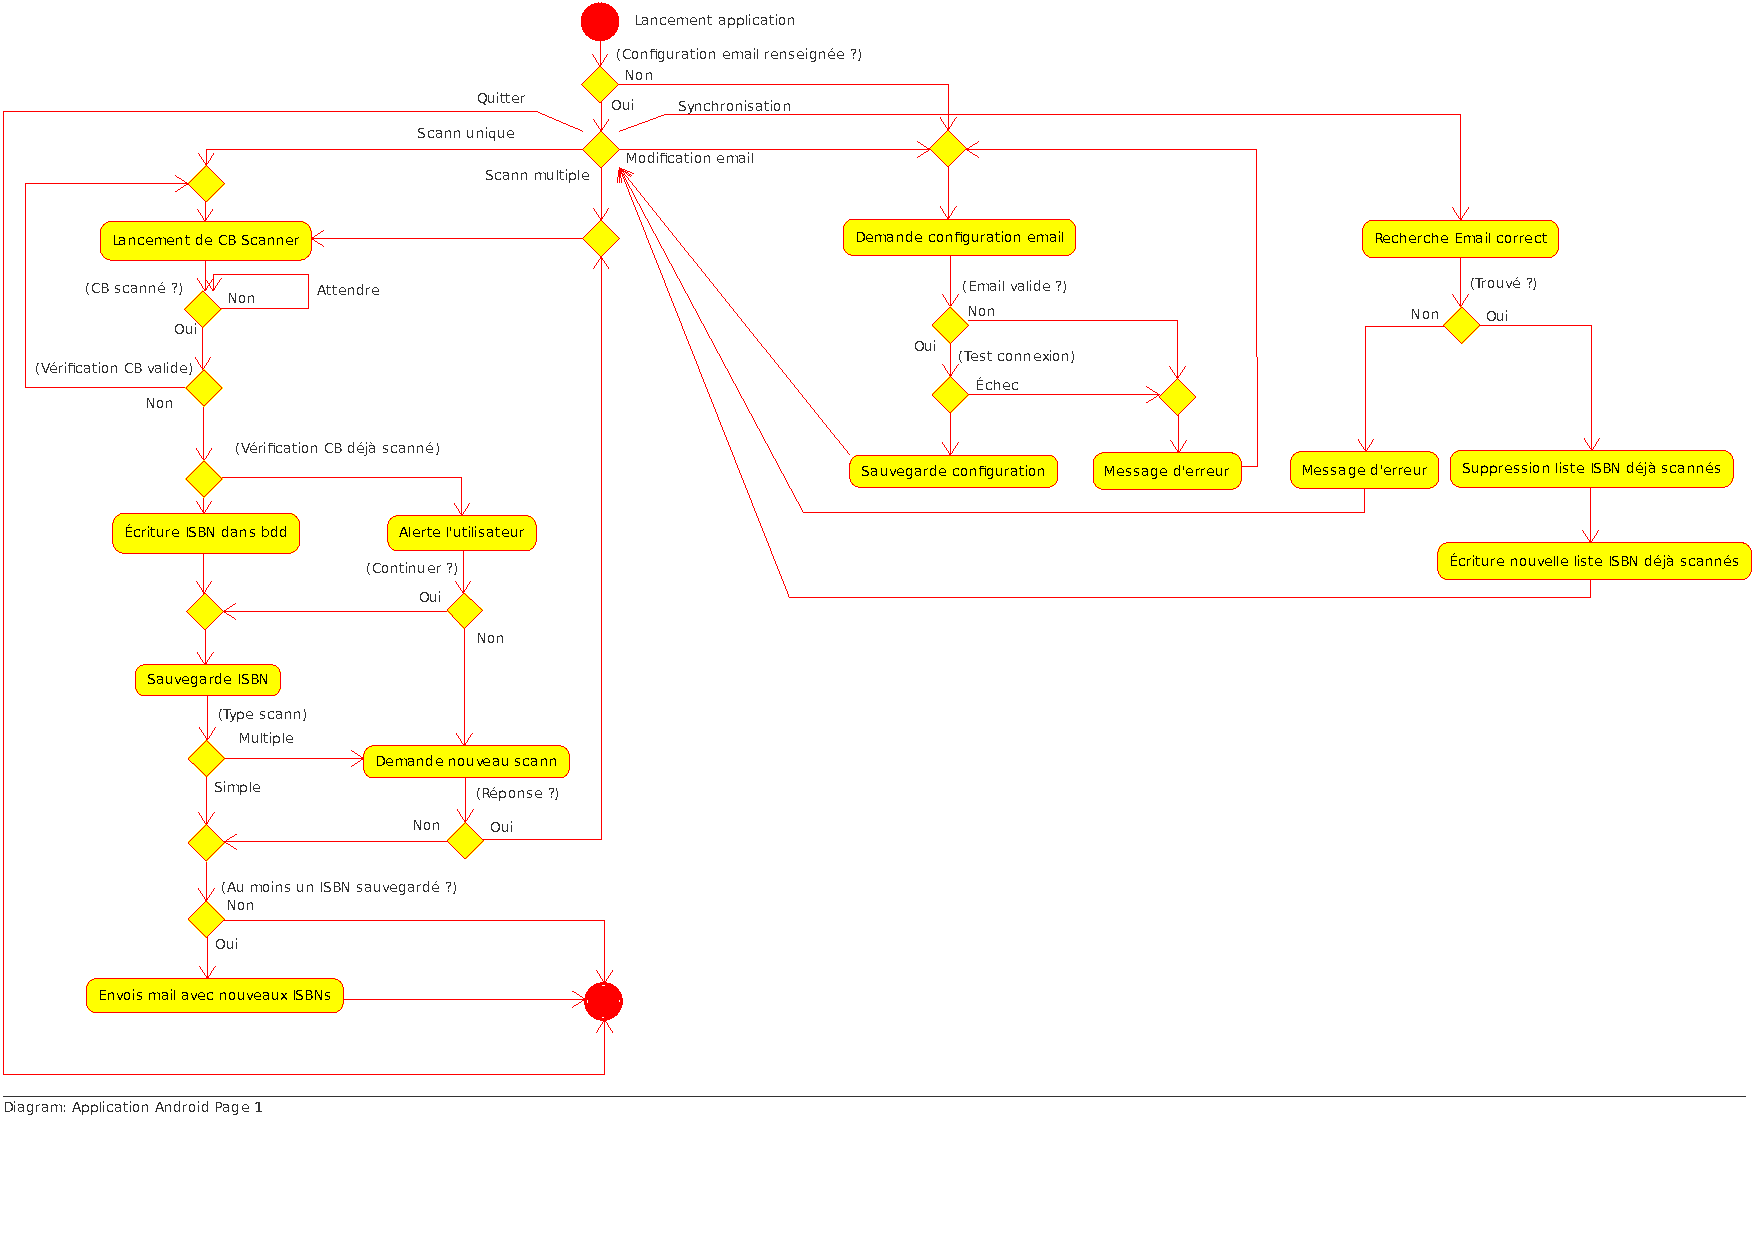
\includegraphics[width=20cm, angle=90]{uml/application_android.pdf}
\end{center}
\end{figure}

